\documentclass[12pt, twoside]{article}
% \documentclass[12pt, twoside]{article}
\usepackage[letterpaper, margin=1in, headsep=0.2in]{geometry}
\setlength{\headheight}{0.6in}
%\usepackage[english]{babel}
\usepackage[utf8]{inputenc}
\usepackage{microtype}
\usepackage{amsmath}
\usepackage{amssymb}
%\usepackage{amsfonts}
\usepackage[nomessages]{fp} %\FPeval{\var-name}{2*sin(pi/6)}
\usepackage{siunitx} %units in math. eg 20\milli\meter
\usepackage{yhmath} % for arcs, overparenth command
\usepackage{tikz} %graphics
\usetikzlibrary{quotes, angles, arrows, arrows.meta}
\usepackage{graphicx} %consider setting \graphicspath{{images/}}
\usepackage{parskip} %no paragraph indent
\usepackage{enumitem}
\usepackage{multicol}
\usepackage{venndiagram}

\usepackage{fancyhdr}
\pagestyle{fancy}
\fancyhf{}
\renewcommand{\headrulewidth}{0pt} % disable the underline of the header
\raggedbottom
\hfuzz=2mm %suppresses overfull box warnings

\usepackage{hyperref}
\usepackage{float}

\title{Algebra 2}
\author{Chris Huson}
\date{November 2024}

\fancyhead[LE]{\thepage}
\fancyhead[RO]{\thepage \\ First and last name: \hspace{2.5cm} \,\\ Section: \hspace{2.5cm} \,}
\fancyhead[LO]{BECA / Huson / Algebra 2: Polynomials \\* 19 November 2024}

\begin{document}

\subsubsection*{3.5 Trimester Final Exam \hfill A2.A.APR.6}
\begin{enumerate}[itemsep=0.5cm]
\subsubsection*{A2-APR.1 Perform operations with polynomials}
\item Find the sum in standard form $(4x^4+5x^3+3x^2-4) + (x^4-2x^3-2x^2-x+1)$. \vspace{8cm}

\item Which expression is equivalent to $(x + 2)^2 - 5(x + 2) + 6$?
    \begin{enumerate}
        \item $x(x - 1)$
        \item $(x - 3)(x + 2)$
        \item $(x - 4)(x + 3)$
        \item $(x - 6)(x + 1)$
    \end{enumerate}
        
\item Which equation represents a polynomial identity? %January 2023 Regents
\begin{enumerate}
    \item \(x^3 + y^3 = (x + y)^3\)
    \item \(x^3 + y^3 = (x + y)(x^2 - xy + y^2)\)
    \item \(x^3 + y^3 = (x + y)(x^2 - xy - y^2)\)
    \item \(x^3 + y^3 = (x - y)(x^2 + xy + y^2)\)
\end{enumerate}

\newpage
\item Write the expression $A(x) \cdot B(x) - 3C(x)$ as a polynomial in standard form. %2 points January 2023 Regents
    \begin{align*}
        A(x) &= x^3 + 2x - 1 \\
        B(x) &= x^2 + 7 \\
        C(x) &= x^4 - 5x
    \end{align*} \vspace{6cm}
    
\item Stone Manufacturing has developed a cost model, $C(x) = 0.18x^3 + 0.02x^2 + 4x + 180$, where $x$ is the number of sprockets sold, in thousands. The sale price can be modeled by $S(x) = 95.4 - 6x$ and the company’s revenue by $R(x) = x \cdot S(x)$. The company profits, $R(x) - C(x)$, could be modeled by %August 2023 Regents
    \begin{enumerate}
        \item $0.18x^3 + 6.02x^2 + 91.4x + 180$
        \item $0.18x^3 - 5.98x^2 - 91.4x + 180$
        \item $-0.18x^3 - 6.02x^2 + 91.4x - 180$
        \item $0.18x^3 + 5.98x^2 + 99.4x + 180$
    \end{enumerate}
    
\newpage
\subsubsection*{A2-F.IF.7a Graph linear and quadratic functions, show key features}
\item One equation of a system is graphed. Graph the second equation, labeling the intersections as ordered pairs.

    \begin{multicols}{2}
      $y = ax^2 - 2x + 9$ \\
      \columnbreak
      $2x + y = 3$
      \end{multicols}
      Find the value of the leading coefficient $a$ of the quadratic equation. \vspace{2cm}
  
    \begin{center}
    \begin{tikzpicture}[scale=.635]
      \draw [help lines] (-10,-10) grid (10,10);
      \draw [thick, ->] (-10.2,0) -- (10.4,0) node [below right] {$x$};
      \draw [thick, ->] (0,-10.2)--(0,10.4) node [left] {$y$};
      \draw[thick, <->,smooth, domain=-4.15:2.85] plot (\x, {-1.5*(\x)^2 - 2*\x + 9});
    \end{tikzpicture}
    \end{center}
  

\newpage
\subsubsection*{A2-A.APR.3 Identify zeros of polynomials given suitable factorizations}
\item Write down the solutions to the equation $x(3x - 1)(x + 5)(x - 1) = 0$. \vspace{2cm} 

\item The polynomial $p$ is a function of $x$. The graph of $p$ has three zeros at $7$, $\frac{2}{3}$, and $-1$. Select $\bf{all}$ the expressions that could represent $p$. \vspace{0.25cm}
    \begin{multicols}{2}
    \begin{enumerate}
        \item $(x-7)(x-\frac{2}{3})(x+1)$
        \item $(x-7)(3x-2)(x-1)$
        \item $3(x-7)(x-\frac{2}{3})(x+1)$
        \item $3x(x+7)(x+\frac{2}{3})(x-1)^2$
        \item $(x-7)(x+\frac{2}{3})(x-1)$
        \item $(x-7)(3x-2)(x+1)$
        \item $3(x-7)(x-\frac{2}{3})(x-1)$
        \item $3x(x+7)(x-\frac{2}{3})(x+1)^2$
    \end{enumerate}
    \end{multicols}
        \vspace{0.5cm}

\subsubsection*{A2-A.APR.3 Rewrite rational expressions in different forms}
\item Select the expression that is equivalent to $\displaystyle \frac{2x^2 + 11x - 21}{x+3}$ for $x \neq -3$.
    \begin{enumerate}
        \item $\displaystyle 2x + 5 - \frac{6}{x + 3}$
        \item $\displaystyle 2x + 17 - \frac{20}{x + 3}$
        \item $\displaystyle 2x + 17 - \frac{36}{x + 3}$
        \item $\displaystyle 2x + 5 - \frac{36}{x + 3}$
    \end{enumerate} \vspace{3cm}

\newpage
\subsubsection*{A2-A.SSE.3c Use the properties of exponents}
\item Identify the expressions that are equal to $\displaystyle \frac{2^2}{2^4}$
    \begin{multicols}{2}
    \begin{enumerate}
        \item $2^6$
        \item $\displaystyle \frac{1}{2^2}$
        \item $2^{-2}$
        \item $\frac{1}{4}$
        \item $2^{2}$
        \item $0.5$
    \end{enumerate}
    \end{multicols}

\item Identify the expressions that are equal to $\displaystyle 2^{-3}$
    \begin{multicols}{2}
    \begin{enumerate}
        \item $2.333...$
        \item $\sqrt{2}$
        \item $\displaystyle \frac{1}{2^3}$
        \item $\displaystyle \frac{1}{8}$
        \item $6$
        \item $0.125$
    \end{enumerate}
    \end{multicols}

\item Identify the expressions that are equal to $\displaystyle 9^{\frac{1}{2}}$
    \begin{multicols}{2}
    \begin{enumerate}
        \item $9.5$
        \item $\sqrt{3}$
        \item $\sqrt{9}$
        \item $3$
        \item $81$
        \item $4.5$
    \end{enumerate}
    \end{multicols}
        
\newpage
\subsubsection*{A2-F.BF.2 Write arithmetic and geometric sequences with recursive formulas}
\item Write a recursive definition of the sequence $a_1 = 2$, $a_2 = 6$, $a_3 = 18$, $a_4 = 54, \ldots$ \vspace{2cm}

\item Write a recursive definition of the arithmetic sequence $a$. \\[0.5cm]
\renewcommand{\arraystretch}{1.5}
\begin{tabular}{|c|c|}
\hline
$n$ & $a_n$ \\
\hline
$1$ & $5$ \\
$2$ & $-5$ \\
$3$ & $-15$ \\
\hline
\end{tabular} \vspace{1cm}

\newpage 
\subsubsection*{A2-F.IF.7c Graph polynomials, identify zeros, end behavior}

\item Graphed is $f(x) = x^3+2x^2-5x-6$. Write the function in factored form. 
    \begin{flushright}
    \begin{tikzpicture}[xscale=1, yscale=0.25]
        \draw [thick, ->] (-3.2,0) -- (4,0) node [above] {$x$};
        \draw [thick, ->] (0,-9.2)--(0,10) node [right] {$y$};
        \foreach \x in {-3,...,3} \draw (\x cm,12pt) -- (\x cm,-12pt) node[below] {$\x$};
        \foreach \y in {-8,-6,4,8} \draw (3pt,\y cm) -- (-3pt,\y cm) node[left] {$\y$};
        \draw [thick, <->,smooth,samples=20,domain=-3.3:2.4] plot(\x,{(\x-2)*(\x+1)*(\x+3)});
    \end{tikzpicture}
    \end{flushright}

\item The graph of the polynomial $f(x) = x^{4}-9x^{2}-4x+12$ is shown. 
    \begin{multicols}{2}
        \begin{enumerate}[itemsep=1cm]
            \item What is the degree of the function?
            \item What are the zeros of the function?
            \item Which factor has a multiplicity of 2?
            \item Write down the $y$-intercept as an ordered pair.
            \item Three points are marked on the graph, $p$, $q$, and $r$. Which one is a local minimum?
        \end{enumerate} \vspace{1cm} \;
    
        \columnbreak
    
        \begin{tikzpicture}[xscale=0.7, yscale=0.8]
            \draw[lightgray,very thin] (-4,-4) grid (4,5);
            \draw [thick, ->] (-4.2,0) -- (4.4,0) node [above] {$x$};
            \draw [thick, ->] (0,-4.2)--(0,5.5) node [right] {$y$};
            \foreach \x in {-4,4} \draw (\x cm,5pt) -- (\x cm,-5pt) node[below] {$\x$};
            \draw (5pt,5 cm) -- (-5pt,5 cm) node[left] {$20$};
            \draw [thick, <->,smooth,samples=20,domain=-3:3.3] plot(\x,{0.25*(\x-1)*(\x-3)*(\x+2)^2});
            \filldraw [black] (-0.27, 3.1) circle (2.5pt) node[above left]{$p$};
            \filldraw [black] (1, 0) circle (2.5pt) node[above right]{$q$};
            \filldraw [black] (2.23, -4.2) circle (2.5pt) node[above]{$r$};

        \end{tikzpicture}
    \end{multicols}

\newpage
\item Let $j(x)= x(x+4)(x-3)^2$ be a polynomial function. 
    \begin{center}
    \begin{tikzpicture}[xscale=0.7, yscale=0.7]
        \draw [thick, ->] (-7.2,0) -- (7.5,0) node [above] {$x$};
        \draw [thick, ->] (0,-6.2)--(0,6.5) node [right] {$y$};
        \foreach \x in {-7,...,7} \draw (\x cm,5pt) -- (\x cm,-5pt);
    \end{tikzpicture}
    \end{center}
    \begin{enumerate}[itemsep=0.25cm]
        \item Sketch a graph of the function. Label the $x$-intercepts.
        \item Find the value of the $y$-intercept and mark it on the graph. \vspace{1cm}
        \item Identify the end behavior of the function.
            \begin{multicols}{2}
            \begin{enumerate}
                \item As $x \to +\infty$, $y \to +\infty$; \\ 
                as $x \to -\infty$, $y \to -\infty$
                \item As $x \to +\infty$, $y \to -\infty$; \\
                as $x \to -\infty$, $y \to +\infty$
                \item As $x \to +\infty$, $y \to +\infty$; \\
                as $x \to -\infty$, $y \to +\infty$
                \item As $x \to +\infty$, $y \to -\infty$; \\
                as $x \to -\infty$, $y \to -\infty$        
            \end{enumerate}
            \end{multicols}
    \end{enumerate}
        
\item Given the rational function $\displaystyle r(x)= \frac{x+3}{x-2}-3$. % F.IF.7d Graph rational functions
        \begin{enumerate}[itemsep=0.25cm]
            \item Sketch a graph of the function.
            \item Mark the vertical asymptote as dotted line and label it with its equation.
            \item Explain why the asymptote is located there.
        \end{enumerate}
        \begin{center}
        \begin{tikzpicture}[xscale=0.7, yscale=0.7]
            \draw [thick, ->] (-8.2,0) -- (8.5,0) node [above] {$x$};
            \draw [thick, ->] (0,-8.2)--(0,8.5) node [right] {$y$};
            \foreach \x in {-8,-6,-4,-2,2,4,6,8} \draw (\x cm,5pt)--(\x cm,-5pt) node at (\x,-0.5){\x};
            \foreach \y in {-8,-6,-4,-2,2,4,6,8} \draw (5pt,\y cm)--(-5pt,\y cm) node at (-0.5,\y){\y};
        \end{tikzpicture}
        \end{center}


\newpage
\subsubsection*{6.EE.b Reason about and solve one-variable equations and inequalities}
% (A.REI.4 Solve quadratic equations algebraically)

\item Use the function $f(x) = \frac{1}{2}x + 11$ to answer the questions.
    \begin{multicols}{2}
    \begin{enumerate}[itemsep=2cm]
        \item Find the value of $f(4)$.
        \item Solve for $x$ if $f(x) = 2$.
    \end{enumerate}
    \end{multicols} \vspace{3cm}

    
\item Solve each equation for $x$.
\begin{multicols}{2}
    \begin{enumerate}
    \item $x^2+5x+6 = 0$
    \item $x^3-7x^2+6x = 0$ 
    \end{enumerate} 
\end{multicols}

 \vspace{4cm}

\item Find all of the values of $x$ that make the equation true. 
$$\frac{3}{x-4} = \frac{x-5}{x}$$ \vspace{4cm}


\item Solve algebraically for $x$: $\displaystyle \frac{1}{x^2} + \frac{1}{2x} = \frac{6}{3x}$ 
\vspace{4cm}

\item Solve algebraically for $n$: $\displaystyle \frac{2}{n^2} + \frac{3}{n} = \frac{4}{n^2}$ %June 2022 Regents
        \vspace{4cm}


\end{enumerate}
\end{document}